\documentclass[12pt]{article}
\usepackage[a4paper]{geometry}
\usepackage[myheadings]{fullpage}
\usepackage{fancyhdr}
\usepackage{lastpage}
\usepackage{graphicx, wrapfig, subcaption, setspace, booktabs}
\usepackage[font=small, labelfont=bf]{caption}
\usepackage{fourier}
\usepackage[protrusion=true, expansion=true]{microtype}
\usepackage[english]{babel}
\usepackage[final]{hyperref} 
\usepackage{sectsty}
\usepackage{cite}
\usepackage{url, lipsum}
\usepackage{float}
\usepackage{amsmath}
\usepackage{mathpazo}
\usepackage{mathtools}
\usepackage{multicol}
\usepackage[none]{hyphenat}
\usepackage{siunitx}
\usepackage[RPvoltages]{circuitikz}
\usepackage{gensymb}
\usepackage[framed,numbered]{matlab-prettifier}
\usepackage{chngcntr}
\usepackage[T1]{fontenc}
\usepackage{tabularx}
\usepackage{minted}

\newcommand{\HRule}[1]{\rule{\linewidth}{#1}}
\newcommand*\mean[1]{\overline{#1}}
\onehalfspacing
\setcounter{tocdepth}{5}
\setcounter{secnumdepth}{5}



%-------------------------------------------------------------------------------
% HEADER & FOOTER
%-------------------------------------------------------------------------------
\pagestyle{fancy}
\fancyhf{}
\setlength\headheight{15pt}
\fancyhead[L]{CSCI403 - Project 3 Part 1}
\fancyhead[R]{Ching}
\fancyfoot[R]{Page \thepage\ of \pageref{LastPage}}
%-------------------------------------------------------------------------------
% TITLE PAGE
%-------------------------------------------------------------------------------
\title{\uppercase{CSCI403 - Project 3 Part 1}}
\author{Brandon Ching}



\begin{document}

\section{Introduction}
The timber problem involves a log of wood that is divided into smaller logs of varying sizes. The goal is to find the maximum amount of timber that can be obtained by an individual. This problem can be solved using a recursive algorithm, which is the focus of this analysis.

\section{Basic Recursive Algorithm}
\begin{minted}[linenos]{python}
def timber_recursive(log_sizes):
    # Base Case
    if len(log_sizes) == 1:
        return log_sizes[0]

    # Recursive Case
    return sum(log_sizes) - min(timber_recursive(log_sizes[1:]),
                                timber_recursive(log_sizes[:-1]))
\end{minted}
\label{timber_recursive}

The timber problem is solvable using a recursive algorithm. With each recursive call, 2 subproblems are created, one with the first log removed and one with the last log removed. Thus the total operations for the recursive algorithm is: $O(2^n)$.

\begin{equation}
    1 + 2 + 2^2 + 2^3 + ... + 2^n = \Theta(2^n)
\end{equation}

\section{Experimental Analysis}
To validate the theoretical analysis, the recursive algorithm presented in Section \ref*{timber_recursive} was implemented in Python \footnote{Simulation ran on Apple M2 Pro with 16GB unified RAM} and tested with various input sizes, $1 \leq n \leq 20$. The python random library was used to generate random log sizes for each input size ranging from 1 to 1000. The algorithm was run 100 times for each size and the average time taken to solve the timber problem was recorded for each input size in Table \ref{tab:timber_recursive_results}.

\subsection{Experimental Results}
\begin{table}[H]
    \caption{Average time taken to solve the timber problem using the recursive algorithm}
    \label{tab:timber_recursive_results}
    \centering
    \begin{tabular}{|c|c|c|c|}
        \hline
        \textbf{Size} & \textbf{Average Time (ms)} & \textbf{Size} & \textbf{Average Time (ms)} \\
        \hline
        1             & 0.000128746                & 11            & 0.286386013                \\ \hline
        2             & 0.00074625                 & 12            & 0.565309525                \\ \hline
        3             & 0.001773834                & 13            & 1.151502132                \\ \hline
        4             & 0.003342628                & 14            & 2.258636951                \\ \hline
        5             & 0.007317066                & 15            & 4.525690079                \\ \hline
        6             & 0.013577938                & 16            & 9.098799229                \\ \hline
        7             & 0.025353432                & 17            & 18.15497398                \\ \hline
        8             & 0.047571659                & 18            & 36.16346121                \\ \hline
        9             & 0.086071491                & 19            & 72.37869978                \\ \hline
        10            & 0.154359341                & 20            & 145.2968574                \\ \hline
    \end{tabular}
\end{table}

\begin{figure}[H]
    \centering
    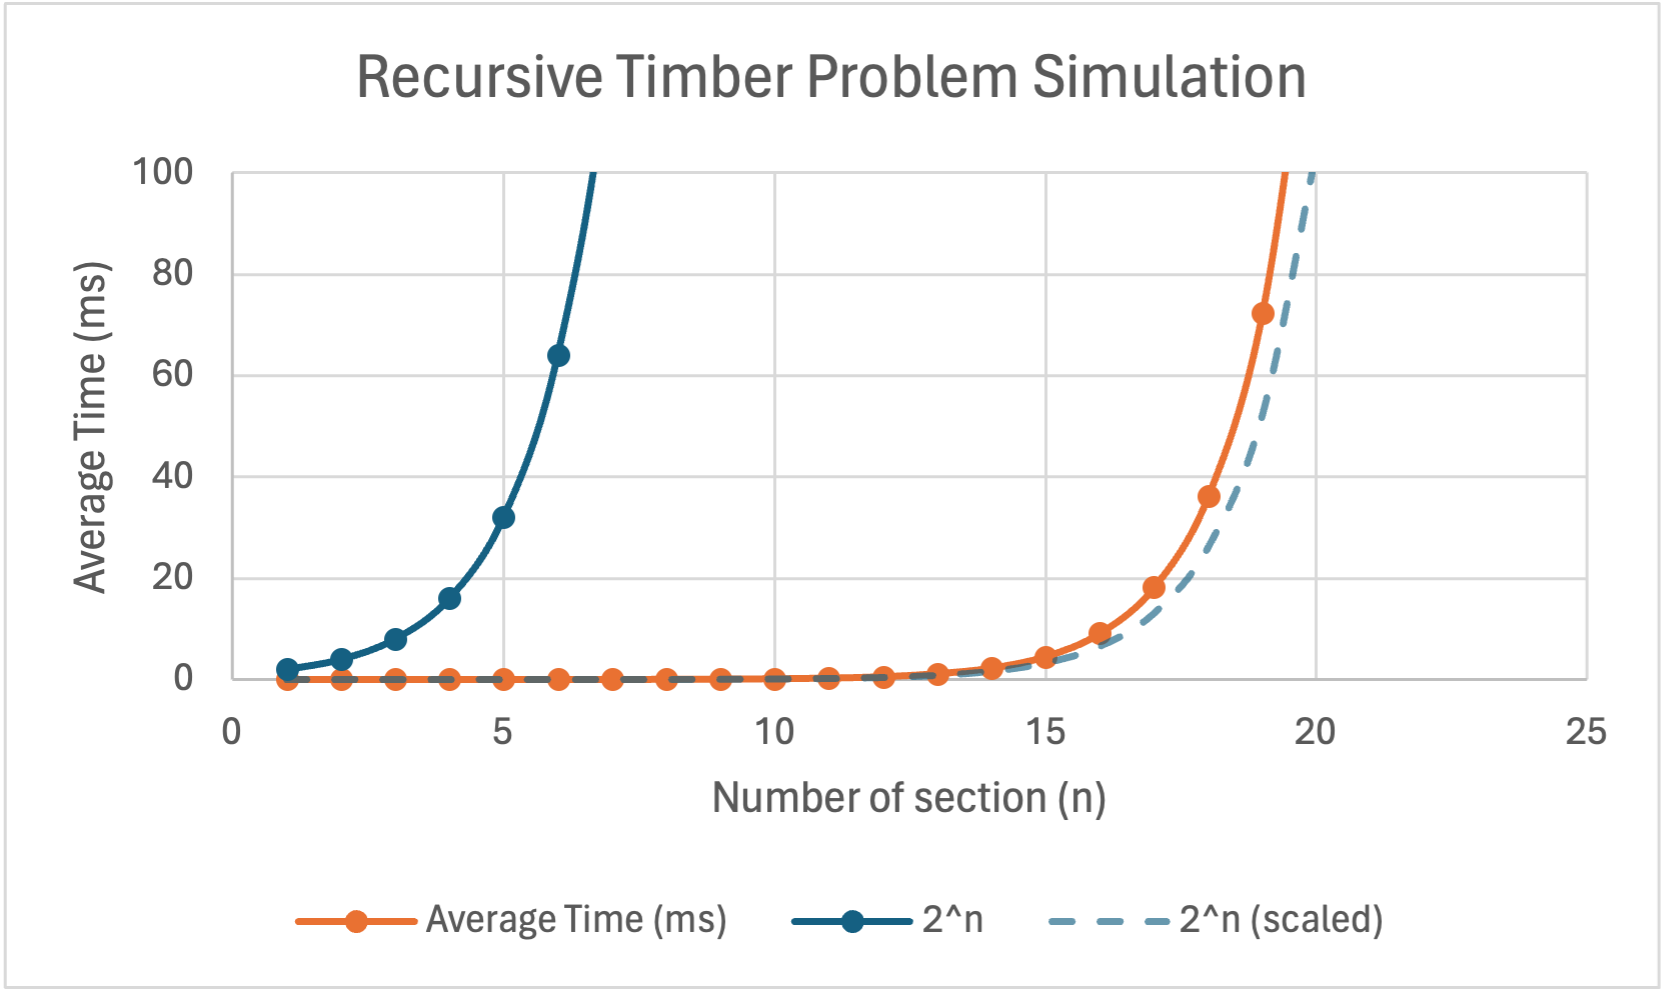
\includegraphics[width=0.8\textwidth]{results_plot.png}
    \caption{Average time taken to solve the timber problem using the recursive algorithm}
    \label{fig:timber_recursive_results}
\end{figure}

\subsection{Analysis}
The experimental results depicted in Table \ref{tab:timber_recursive_results} and Figure \ref{fig:timber_recursive_results} showcase a clear trend: the average time taken to solve the timber problem using the recursive algorithm grows exponentially with the input size. This observation aligns well with the recursive analysis, which predicts a time complexity of $\Theta (2^n)$.

As shown in Figure \ref{fig:timber_recursive_results}, the experimental data closely follows the theoretical analysis of $\Theta(2^n)$ \footnote{To provide a more illustrative comparison, a scaled line representing the theoretical complexity ($\Theta(2^n)$) is included in Figure \ref{fig:timber_recursive_results}. This scaled line, reduced by a factor of 10,000.}. Despite minor fluctuations in runtime, likely attributable to system variations and other factors, the overall trend exhibits exponential growth, confirming the scalability characteristics anticipated by the theoretical analysis.


\section{Appendix - Python Code}

\begin{figure}[H]
    \begin{minted}[linenos]{python}
import sys
import random
import time

def timber_recursive(log_sizes):
    # Base Case
    if len(log_sizes) == 1:
        return log_sizes[0]

    # Recursive Case
    return sum(log_sizes) - min(timber_recursive(log_sizes[1:]),
                                timber_recursive(log_sizes[:-1]))

def synthetic_test():
    # Test all log sizes from 1 to 20. Log files to an output file
    # Use a random number generator to generate the log sizes
    with open("output.csv", "w") as f:
        for i in range(1, 21):
            for j in range(100):
                log_sizes = [random.randint(1, 1001) for _ in range(i)]
                # Run and time the recursive algorithm
                start_time = time.time()
                timber_recursive(log_sizes)
                end_time = time.time()
                time_taken = (end_time - start_time) * 1000
                # Write the results to the output file
                f.write(f"{i}, {timber_recursive(log_sizes)}, {time_taken}\n")

    f.close()

if __name__ == "__main__":
    synthetic_test()
    \end{minted}

\end{figure}



\end{document}